% Foliensatz: "AFu-Kurs nach DJ4UF" von DK0TU, Amateurfunkgruppe der TU Berlin
% Lizenz: CC BY-NC-SA 3.0 de (http://creativecommons.org/licenses/by-nc-sa/3.0/de/)
% Autoren: Sebastian Lange <dl7bst@dk0tu.de>
% Korrekturen: Lars Weiler <dc4lw@darc.de>

\documentclass[aspectratio=169]{beamer}

\usepackage[ngerman]{babel} % deutsche Worttrennung etc.
\usepackage[utf8]{inputenc} % UTF8 Text

\usepackage[super, comma, numbers, square, sort]{natbib}

\usepackage{hyperref}       % Hyperref Package für bessere Referenzen (todo)
\hypersetup{
	colorlinks=false,       %   false: boxed links; true: colored links
    %linkcolor=white,       %   color of internal links (change box color with linkbordercolor)
    citecolor=red,          %   color of links to bibliography
    filecolor=white,        %   color of file links
    urlcolor=blue           %   color of external links
}

\usepackage{multirow}
\usepackage{wasysym}  % Math Symbols like \permil
%\usepackage{colortbl}
%\usepackage{subscript}
%\usepackage{caption}
%\usepackage{setspace}
%\usepackage{xcolor}        % benutze CodeListe

% Footnote
%\usepackage{hanging}
%
%\setbeamertemplate{footnote}{%
%  \hangpara{2em}{1}%
%  \makebox[2em][l]{\insertfootnotemark}\footnotesize\insertfootnotetext\par%
%}


%\usepackage{pgf}
%\usepackage{tikz}
%\usetikzlibrary{arrows,automata}
%\usetikzlibrary{positioning}
%
%\tikzset{
%    state/.style={
%           rectangle,
%           rounded corners,
%           draw=black, very thick,
%           minimum height=2em,
%           minimum width=2pt,
%           inner sep=2pt,
%           text centered,
%           },
%}

%\usepackage{listings}
%\lstset{basicstyle=\small, numberstyle=\tiny, extendedchars=true, numbers=left, numbersep=5pt}
%\lstset{showtabs=false, showspaces=false, showstringspaces=false}
%%\lstset{backgroundcolor=\color{white!75!lightgray}, , frame=single}
%%\lstset{backgroundcolor=\color{white}}
%%\lstset{backgroundcolor=none}
%\lstset{keywordstyle=\color{blue!50!gray},  identifierstyle=\color{black}}
%\lstset{commentstyle=\color{green!50!gray}, stringstyle=\color{red!50!gray}}
%\lstset{language=C, fontadjust=true, tabsize=2, breaklines=true}
%\lstset{backgroundcolor=\color{white!75!lightgray}, caption=\lstname, frame=single}
%\lstset{emphstyle=\color{black}\fbox}
%
%% Keine "Listing:"-Caption
%\captionsetup{labelformat=empty,labelsep=none}
%
%% für mathematische Umgebungen
%\usepackage{amsmath,amsfonts,amssymb}
%
%\lstdefinestyle{Bash}{
%language=Bash,
%frame=single,
%rulecolor=\color{black},
%backgroundcolor=\color{gray!50},
%keywordstyle=\color{black},
%identifierstyle=,
%commentstyle=\color{black},
%stringstyle=\color{magenta!65!white},
%showstringspaces=false,
%basicstyle=\footnotesize\ttfamily\color{black},
%numbers=none,
%breaklines=true,
%captionpos=b
%}

%\usepackage{listings}
%
%\lstdefinestyle{basic}{
%    captionpos=t,%
%    basicstyle=\footnotesize\ttfamily,%
%    numberstyle=\tiny,%
%    numbers=left,%
%    stepnumber=1,%
%    frame=single,%
%    showspaces=false,%
%    showstringspaces=false,%
%    showtabs=false,%
%    %
%    keywordstyle=\color{blue},%
%    identifierstyle=,%
%    commentstyle=\color{gray},%
%    stringstyle=\color{magenta}%
%}



% fließende Boxen haben keinen Abstand
%\fboxsep0mm

% inkludiere Creative Commons Helper
%%%%%%%%%%%%%%%%%%%%%%%%%%%%%%%%%%%%%%%%%%%%%%%%%%%%%%%%%%%%%%%%
%% ccBeamer 0.1, 2007-07-02                                   %%
%% Written by Sebastian Pipping <webmaster@hartwork.org>      %%
%% ---------------------------------------------------------- %%
%% Licensed under Creative Commons Attribution-ShareAlike 3.0 %%
%% http://creativecommons.org/licenses/by-sa/3.0/             %%
%%%%%%%%%%%%%%%%%%%%%%%%%%%%%%%%%%%%%%%%%%%%%%%%%%%%%%%%%%%%%%%%


%% Images
\newcommand{\CcImageBy}[1]{%
	
\includegraphics[scale=#1]{texdata/creative_commons/cc_by_30.pdf}%
}
\newcommand{\CcImageCc}[1]{%
	
\includegraphics[scale=#1]{texdata/creative_commons/cc_cc_30.pdf}%
}
\newcommand{\CcImageDevNations}[1]{%
	
\includegraphics[scale=#1]{texdata/creative_commons/cc_dev_nations_30.pdf}%
}
\newcommand{\CcImageNc}[1]{%
	
\includegraphics[scale=#1]{texdata/creative_commons/cc_nc_30.pdf}%
}
\newcommand{\CcImageNd}[1]{%
	
\includegraphics[scale=#1]{texdata/creative_commons/cc_nd_30.pdf}%
}
\newcommand{\CcImagePd}[1]{%
	
\includegraphics[scale=#1]{texdata/creative_commons/cc_pd_30.pdf}%
}
\newcommand{\CcImageSa}[1]{%
	
\includegraphics[scale=#1]{texdata/creative_commons/cc_sa_30.pdf}%
}
\newcommand{\CcImageSampling}[1]{%
	
\includegraphics[scale=#1]{texdata/creative_commons/cc_sampling_30.pdf}%
}
\newcommand{\CcImageSamplingPlus}[1]{%
	
\includegraphics[scale=#1]{texdata/creative_commons/cc_sampling_plus_30.pdf}%
}


%% Groups
\newcommand{\CcGroupBy}[2]{% zoom, gap
	\CcImageCc{#1}\hspace*{#2}\CcImageBy{#1}%
}
\newcommand{\CcGroupByNc}[2]{% zoom, gap
	\CcImageCc{#1}\hspace*{#2}\CcImageBy{#1}\hspace*{#2}\CcImageNc{#1}%
}
\newcommand{\CcGroupByNcNd}[2]{% zoom, gap
	\CcImageCc{#1}\hspace*{#2}\CcImageBy{#1}\hspace*{#2}\CcImageNc{#1}\hspace*{#2}\CcImageNd{#1}%
}
\newcommand{\CcGroupByNcSa}[2]{% zoom, gap
	\CcImageCc{#1}\hspace*{#2}\CcImageBy{#1}\hspace*{#2}\CcImageNc{#1}\hspace*{#2}\CcImageSa{#1}%
}
\newcommand{\CcGroupByNd}[2]{% zoom, gap
	\CcImageCc{#1}\hspace*{#2}\CcImageBy{#1}\hspace*{#2}\CcImageNd{#1}%
}
\newcommand{\CcGroupBySa}[2]{% zoom, gap
	\CcImageCc{#1}\hspace*{#2}\CcImageBy{#1}\hspace*{#2}\CcImageSa{#1}%
}
\newcommand{\CcGroupDevNations}[2]{% zoom, gap
	\CcImageCc{#1}\hspace*{#2}\CcImageDevNations{#1}%
}
\newcommand{\CcGroupNcSampling}[2]{% zoom, gap
	\CcImageCc{#1}\hspace*{#2}\CcImageNc{#1}\hspace*{#2}\CcImageSampling{#1}%
}
\newcommand{\CcGroupPd}[1]{% zoom
	\CcImagePd{#1}%
}
\newcommand{\CcGroupSampling}[1]{% zoom
	\CcImageSampling{#1}%
}
\newcommand{\CcGroupSamplingPlus}[1]{% zoom
	\CcImageSamplingPlus{#1}%
}


%% Text
\newcommand{\CcLongnameBy}{Attribution}
\newcommand{\CcLongnameByNc}{Attribution-NonCommercial}
\newcommand{\CcLongnameByNcNd}{Attribution-NoDerivs}
\newcommand{\CcLongnameByNcSa}{Attribution-NonCommercial-ShareAlike}
\newcommand{\CcLongnameByNd}{Attribution-NoDerivs}
\newcommand{\CcLongnameBySa}{Attribution-ShareAlike}

\newcommand{\CcNote}[1]{% longname
	This work is licensed under the \textit{Creative Commons #1 3.0 License}.%
}


% generelles Thema auswählen
\usetheme{Goettingen} %Berlin spart ohne Sidebar allerdings angenehm Platz
% AnnArbor | Antibes | Bergen | Berkeley | Berlin | Boadilla | boxes | CambridgeUS | Copenhagen | Darmstadt | default | Dresden | Frankfurt | Goettingen | Hannover | Ilmenau | JuanLesPins | Luebeck | Madrid | Malmoe | Marburg | Montpellier | PaloAlto | Pittsburgh | Rochester | Singapore | Szeged | Warsaw

% Farben wählen
\usecolortheme{beetle}
% beaver | beetle | crane | default | dolphin | dove | fly | lily | orchid | rose | seagull | seahorse | sidebartab | structure | whale | wolverine

% Setze alle Farben auf Grau und Weiß
%\definecolor{craneorange}{RGB}{64,64,64}
%\definecolor{craneblue}{RGB}{255,255,255}

% Schriftart wählen
\usefonttheme{default}
% default | professionalfonts | serif | structurebold | structureitalicserif | structuresmallcapsserif

% Innere Themen(Kopf-, Fuß-, Sidebar usw)
%\useinnertheme{default}
\useinnertheme{circles}
% default | inmargin | rectangles | rounded | circles

% Äußere Themen (Anordnung der inneren, grenzen der Folien etc.)
\useoutertheme{infolines}
% default | infolines | miniframes | shadow | sidebar | smoothbars | smoothtree | split | tree

% Deaktiviere Navigations-Symbole ({} -> leer)
\setbeamertemplate{navigation symbols}{}
%\setbeamertemplate{navigation symbols}{\large \ifnum \insertframenumber <10 0\fi\insertframenumber/\inserttotalframenumber\vspace*{0.2ex}}

% Zeige ein Hintergrundbild
\setbeamertemplate{background canvas}{
        \hspace*{-2.0cm}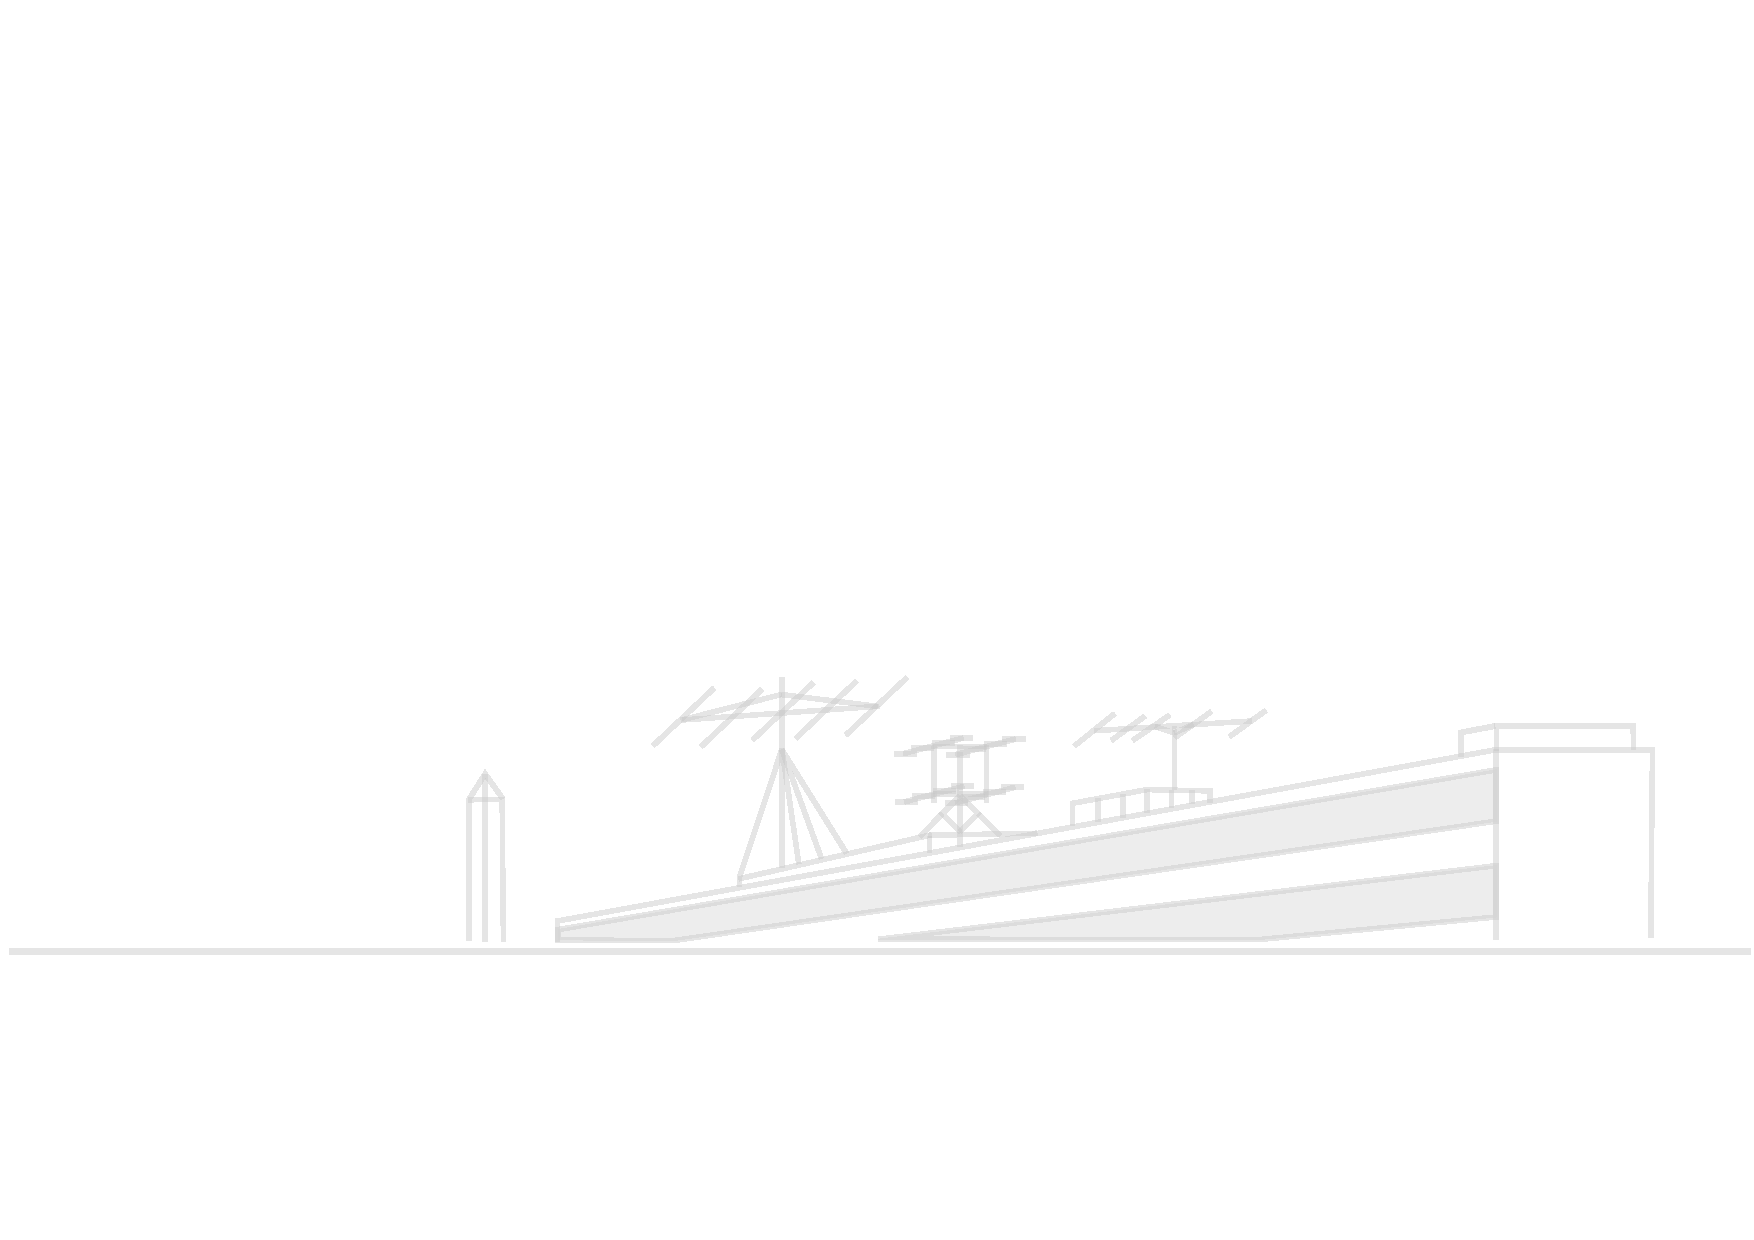
\includegraphics[width=17.8cm]{texdata/dk0tu_rooftop_background.pdf}
}

% Foliennummer einfügen
\setbeamertemplate{footline}[frame number]
%\setbeamertemplate{footline}{}

% Ändere das Zeichen vor jedem item
%\setbeamertemplate{itemize item}{\color{craneorange}$\blacktriangleright$}
%\setbeamertemplate{itemize subitem}{\color{craneorange}$\triangleright$}
%\setbeamertemplate{itemize subsubitem}{\color{craneorange}$\blacktriangleright$}

% Ändert die Blöcke 
\setbeamertemplate{blocks}[rounded][shadow=true]
% default | rounded [shadow=true|false]

%
% Eigene Kommandos
%

% Hack to get natbib and beamer working together. "The beamer user guide suggests
% that only the manual bibliography entry approach is supported"
% on some system it works out of the box, sometimes you need the hack :-(
% so check it --dl7bst
\ifdefined\newblock
    \relax
\else
    \newcommand{\newblock}{}
\fi

% \includedia command to generate png out of a dia file
% NEEDS installed dia and pdflatex option --shell-escape
\newcommand{\includedia}[1]{
    \immediate\write18{/usr/bin/dia #1.dia -e #1_diatmp.png -t png}
}

% RICHIG GROSSER FONT!
\newfont{\bigfont}{cmr10 at 144pt}
\newfont{\smallfont}{cmr10 at 8pt}

% Römische Ziffern
\makeatletter
\newcommand{\rmnum}[1]{\romannumeral #1}
\newcommand{\Rmnum}[1]{\expandafter\@slowromancap\romannumeral #1@}
\makeatother

% Schwarze Überschrift
%\setbeamercolor{frametitle}{fg=black}
%\setbeamercolor{title}{fg=black}

% Item- und Box-Farben
\definecolor{deepBlue}{HTML}{000066}
\setbeamercolor{itemize item}{fg=deepBlue}
\setbeamercolor{itemize subitem}{fg=deepBlue}
\setbeamercolor{description item}{fg=deepBlue}
\setbeamercolor{block title}{fg=deepBlue!100, bg=blue!15}
\setbeamercolor{block body}{fg=black, bg=blue!5}
\setbeamercolor{block title alerted}{fg=deepBlue, bg=red!75}
\setbeamercolor{block body alerted}{fg=black, bg=red!15}
\setbeamercolor*{block title example}{fg=blue!50, bg=blue!10}
\setbeamercolor*{block body example}{fg= blue, bg=blue!5}

%\setbeamercolor{section in head/foot}{parent=palette primary}
%\setbeamercolor{subsection in head/foot}{parent=palette secondary}
%\setbeamercolor{sidebar}{fg=darkblue,bg=yellow!90!orange}
%\setbeamercolor{title in sidebar}{fg=darkblue}
%\setbeamercolor{author in sidebar}{fg=darkblue}
%\setbeamercolor{section in sidebar}{fg=darkblue!10!black}
%\setbeamercolor{subsection in sidebar}{fg=darkblue!50!black}

% Titlepage Infos
\title{AFu-Kurs nach DJ4UF}
\author[DKØTU]{DKØTU\\ \footnotesize{Amateurfunkgruppe der TU Berlin}}
\institute[DKØTU]{\url{http://www.dk0tu.de} }

% PDF-Eigenschaften
\subject{DK0TU-Amateurfunkkurs nach DJ4UF}
\keywords{Amateurfunk Kurs HAM Radio Course CC-BY-NC-SA OpenSource TU Berlin DK0TU}

\subtitle{Technik Klasse E 16 \& Betriebstechnik/Vorschriften 12: \\
          (Digitale) Betriebsarten \\[2em]}
\date{Stand 14.01.2016}
 \begin{document}

\begin{frame}
    \titlepage
    \vfill
    \begin{center}
        \ccbyncsaeu\\
        {\tiny This work is licensed under the \em{Creative Commons Attribution-NonCommercial-ShareAlike 3.0 License}.}\\[0.5ex]
         \tiny Amateurfunkgruppe der Technische Universität Berlin (AfuTUB), DKØTU
         %\includegraphics[scale=0.5]{img/DK0TU_Logo.pdf}
    \end{center}
\end{frame}


% todo Gern noch mehr Bilder - es ist ein schönes praktisches Thema.
% todo bei viel Text Buzzwords fett hervorheben oder Text kürzen
% todo da der Talk ca. 2h lang ist: Guten Pausenzeitpunkt finden
% todo Eine schöne Datenbank an Digisounds: http://www.nonstopsystems.com/radio/radio-sounds.html
% todo Audioquiz am Ende
% todo Spektrum nochmal mit Audacity/GNU Radio

\section{Einleitung}

\begin{frame}
    \frametitle{Einleitung / Umleitung}

    Aufgrund sehr großer inhaltlicher Überschneidungen der beiden
    \emph{Moltrecht}-Lektionen, ist die Lektion
    \texttt{BV12}\hyperlink{refs}{\cite{bv12}} in diesen Foliensatz der Lektion
    \texttt{Technik E16}\hyperlink{refs}{\cite{e16}} integriert. \\[2em]

    Freut euch auf eine Lektion ``Klingeln in den Ohren'' :-)

\end{frame}

\begin{frame}
    \frametitle{Einleitung / Betriebsarten}

    Grundsätzlich unterscheidet man zwischen:

    \begin{itemize}
		\item analoge Betriebsarten
		\item digitale Betriebsarten (Digimodes)
    \end{itemize}

    Vorweg: In der \emph{Klasse E} liegt der Fokus auf das Kennenlernen und
    betriebstechnische Grundlagen. Die technischen Grundlagen werden dann im
    Technikteil der \emph{Klasse A} ausgebaut.

\end{frame}

\section{analog}

\subsection[Sprechfunk]{Sprechfunk (Wiederholung)}

\begin{frame}
    \frametitle{Sprechfunk (Wiederholung)}

    In Lektion \texttt{E14} wurde das Thema bereits besprochen.

    Der Vollständigkeit halber seien sie noch einmal erwähnt - auch weil die
    meisten Digimodes im Amateurfunk \emph{SSB} oder \emph{FM} als Hauptträger
    benutzen.

\end{frame}

\begin{frame}
    \frametitle{Sprechfunk (Wdh.) / SSB}

    \begin{center}
        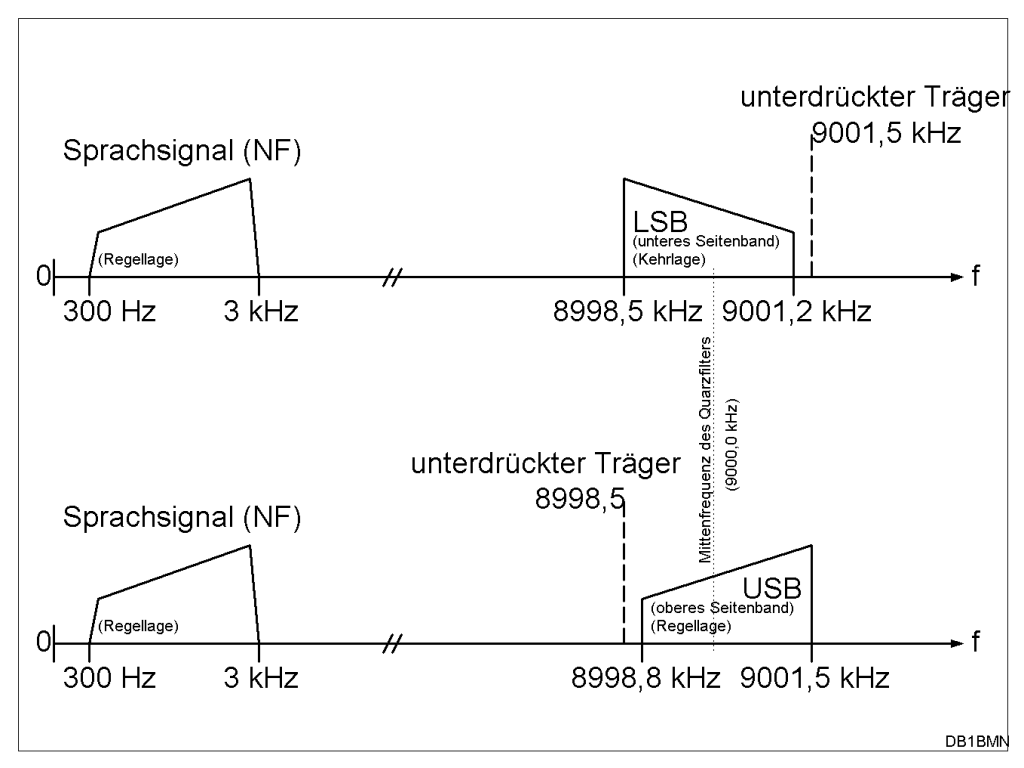
\includegraphics[width=0.8\textwidth,height=.65\textheight,keepaspectratio]{e16/Ssb-de.png}
        \tiny \hyperlink{refs}{\cite{wc}}
    \end{center}

    Durchgängiges (da analoges) Spektrum ca. $300 Hz$ bis $3 kHz$

\end{frame}

\begin{frame}
    \frametitle{Sprechfunk (Wdh.) / FM}

    \begin{center}
        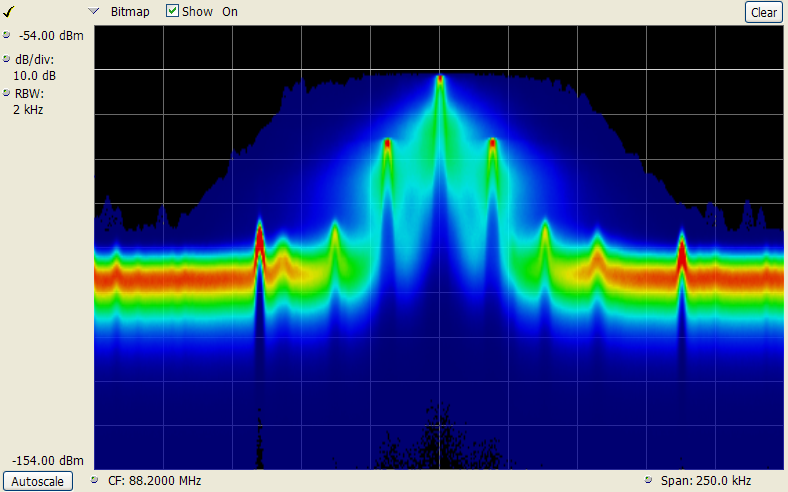
\includegraphics[width=0.8\textwidth,height=.55\textheight,keepaspectratio]{e16/Dpx-fm-radio.png}
        \tiny \hyperlink{refs}{\cite{wc}}
    \end{center}

    Je $2x$ Hub ($3 kHz$) + NF-Signal ($2,7 kHz$) um Träger herum
    (durchgängiges Spektrum) \\[1em]
    
    $\rightarrow$ Gesamtbandbreite eines NBFM-Signals ca. $12 kHz$ ($12,5 kHz$
    Kanalraster)

\end{frame}

\subsection[Hell]{Hellschreiber}
\begin{frame}
  \frametitle{Hellschreiber\,/\,Typenbildfernschreiber}
  \begin{itemize}
    \item 1929 von Rudolf Hell patentiert
    \item Fernschreibgerät für störanfällige Übertragungen
    \item Verwendung bis in die 1980er Jahre
  \end{itemize}
  \begin{center}
    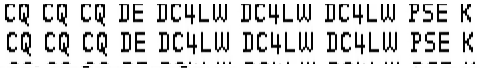
\includegraphics[width=.5\textwidth,height=.3\textheight,keepaspectratio]{e16/Hellschreiber.png}
  \end{center}
  \begin{itemize}
    \item Schriftzeichen im Raster von 7x7 Pixeln
    \item 8,5 Zeichen (in einer Spalte) pro Sekunde (420bit/s)
    \item Bei der Decodiderung wird eine Schneckenwalze auf Papierband gedrückt
    \item zwei Zeilen pro Schnecke; bei Asynchronität verläuft das Schriftbild
  \end{itemize}
  Action: \url{https://www.youtube.com/watch?v=luc6QmNyPZ4}
\end{frame}

\subsection[SSTV]{Slow Scan Television (SSTV)}

\begin{frame}
    \frametitle{SSTV / Historie}

    \textbf{S}low \textbf{S}can \textbf{T}elevision\\[1.5em]

    \begin{columns}[c]
        \column[c]{7cm}
        \begin{itemize}
            \item 1958 durch US-HAMs veröffentlicht
            \item Übertragung von Bildern in $3 kHz$ SSB-Kanal
            \item damals noch Darstellung auf Katodenstrahlröhre mit hoher Nachleuchtdauer
            \begin{itemize}
                \item 120x120 Bildpunkte (s/w) in acht Sekunden
                \item \emph{elektromechanischer SSTV-Empfänger} siehe \texttt{GIF}
                      \href{https://upload.wikimedia.org/wikipedia/commons/1/1e/Mechanical_glow_drum_slow_scan_television_monitor.gif}{[Link]}
            \end{itemize}
        \end{itemize}
        \column{6cm}
        \begin{center}
            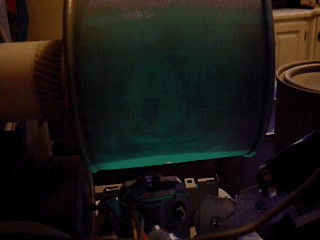
\includegraphics[width=.9\textwidth]{e16/Mechanical_glow_drum_slow_scan_television_monitor.jpg}
            \tiny \hyperlink{refs}{\cite{wc}}
        \end{center}
    \end{columns}

\end{frame}

\begin{frame}
    \frametitle{SSTV / Technik}

    \begin{center}
        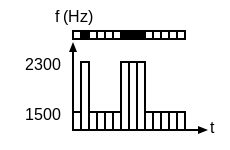
\includegraphics[width=0.4\textwidth]{e16/Sstv_frequences.png}
        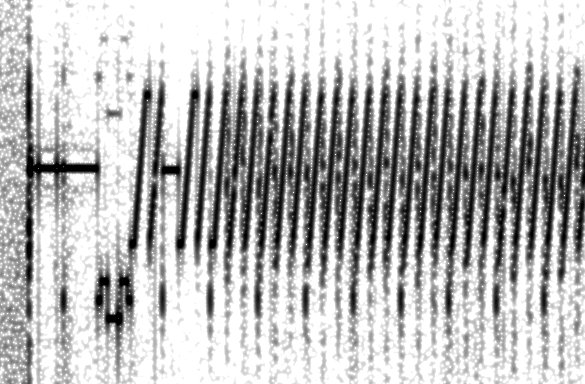
\includegraphics[width=0.4\textwidth]{e16/SSTV_signal.jpg}
        \tiny \hyperlink{refs}{\cite{wc}}
    \end{center}

    \begin{itemize}%[<+->]
        \item heute Software-MODEM via Soundkarte
        \begin{itemize}
            \item Quasi-Standard: 320x240 Bildpunkte (RGB) in 120s
            \item zunehmend ziehen digitale Verfahren mit Fehlerkorrektur ein,
                  z.B. \emph{MT63}\hyperlink{refs}{\cite{wp}}
        \end{itemize}
        \item SSTV-Norm: NF-Frequenz 2300 Hz weiß, 1500 Hertz schwarz, 1200 Hz Sync
        \item am Bildsynchronisierimpuls kann man Modulation erkennen
    \end{itemize}

\end{frame}

\begin{frame}
    \frametitle{SSTV / Betriebstechnik}

    \begin{center}
        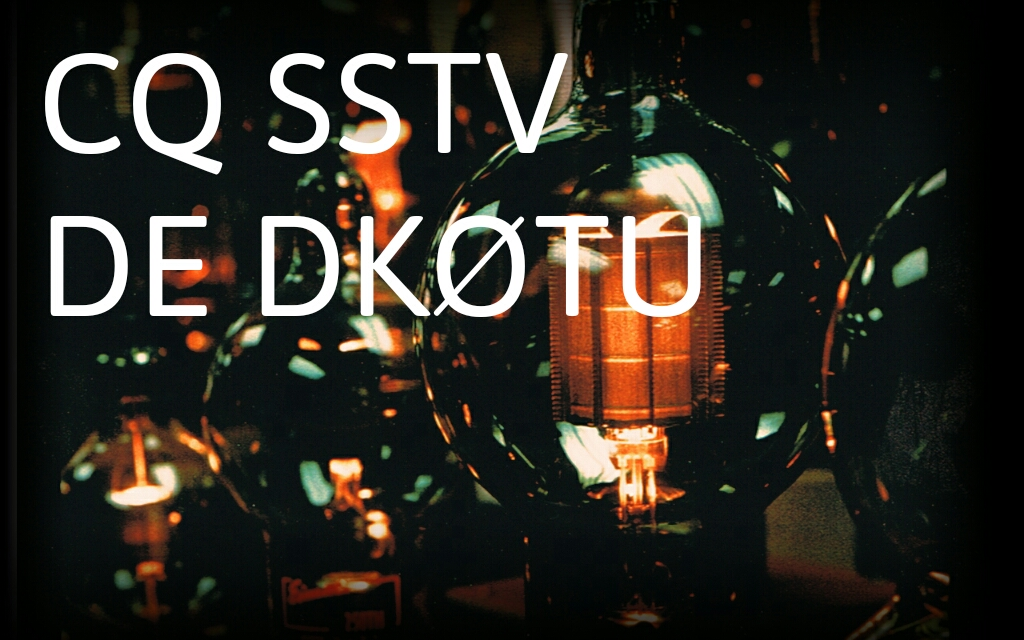
\includegraphics[width=0.7\textwidth,height=.7\textheight,keepaspectratio]{e16/Transmittingtubes.jpg}
    \end{center}

    %todo ordentliche QSL-Karte (Kontrast, Textgröße etc) und Antwort einfügen

    \begin{itemize}
        \item Nachricht meist Fotos von der Funkstation und Text im Bild codiert
    \end{itemize}

\end{frame}

\begin{frame}
    \frametitle{SSTV / Rapportsystem}
   
    %todo Anmerkung: Rapportsystem kommt erst in BV13 dran - Foto einfügen?

    Rapportsystem \textbf{RSV}\hyperlink{refs}{\cite{bv12}}: Readability, Signal Strength, Video

    \begin{itemize}
        \item V1 = Nur Synchronisation zu sehen
        \item V2 = Großes Call lesbar
        \item V3 = Große Details zu erkennen
        \item V4 = Kleine Details zu erkennen
        \item V5 = rauschfreies Bild
    \end{itemize}

    Rapport wird ebenfalls im Bild eingefügt $\rightarrow$ siehe DKØTU
    SSTV-RX-Sammlung

\end{frame}

\begin{frame}
    \frametitle{SSTV / ``NF over Ackerschnacker''}

    \begin{center}
        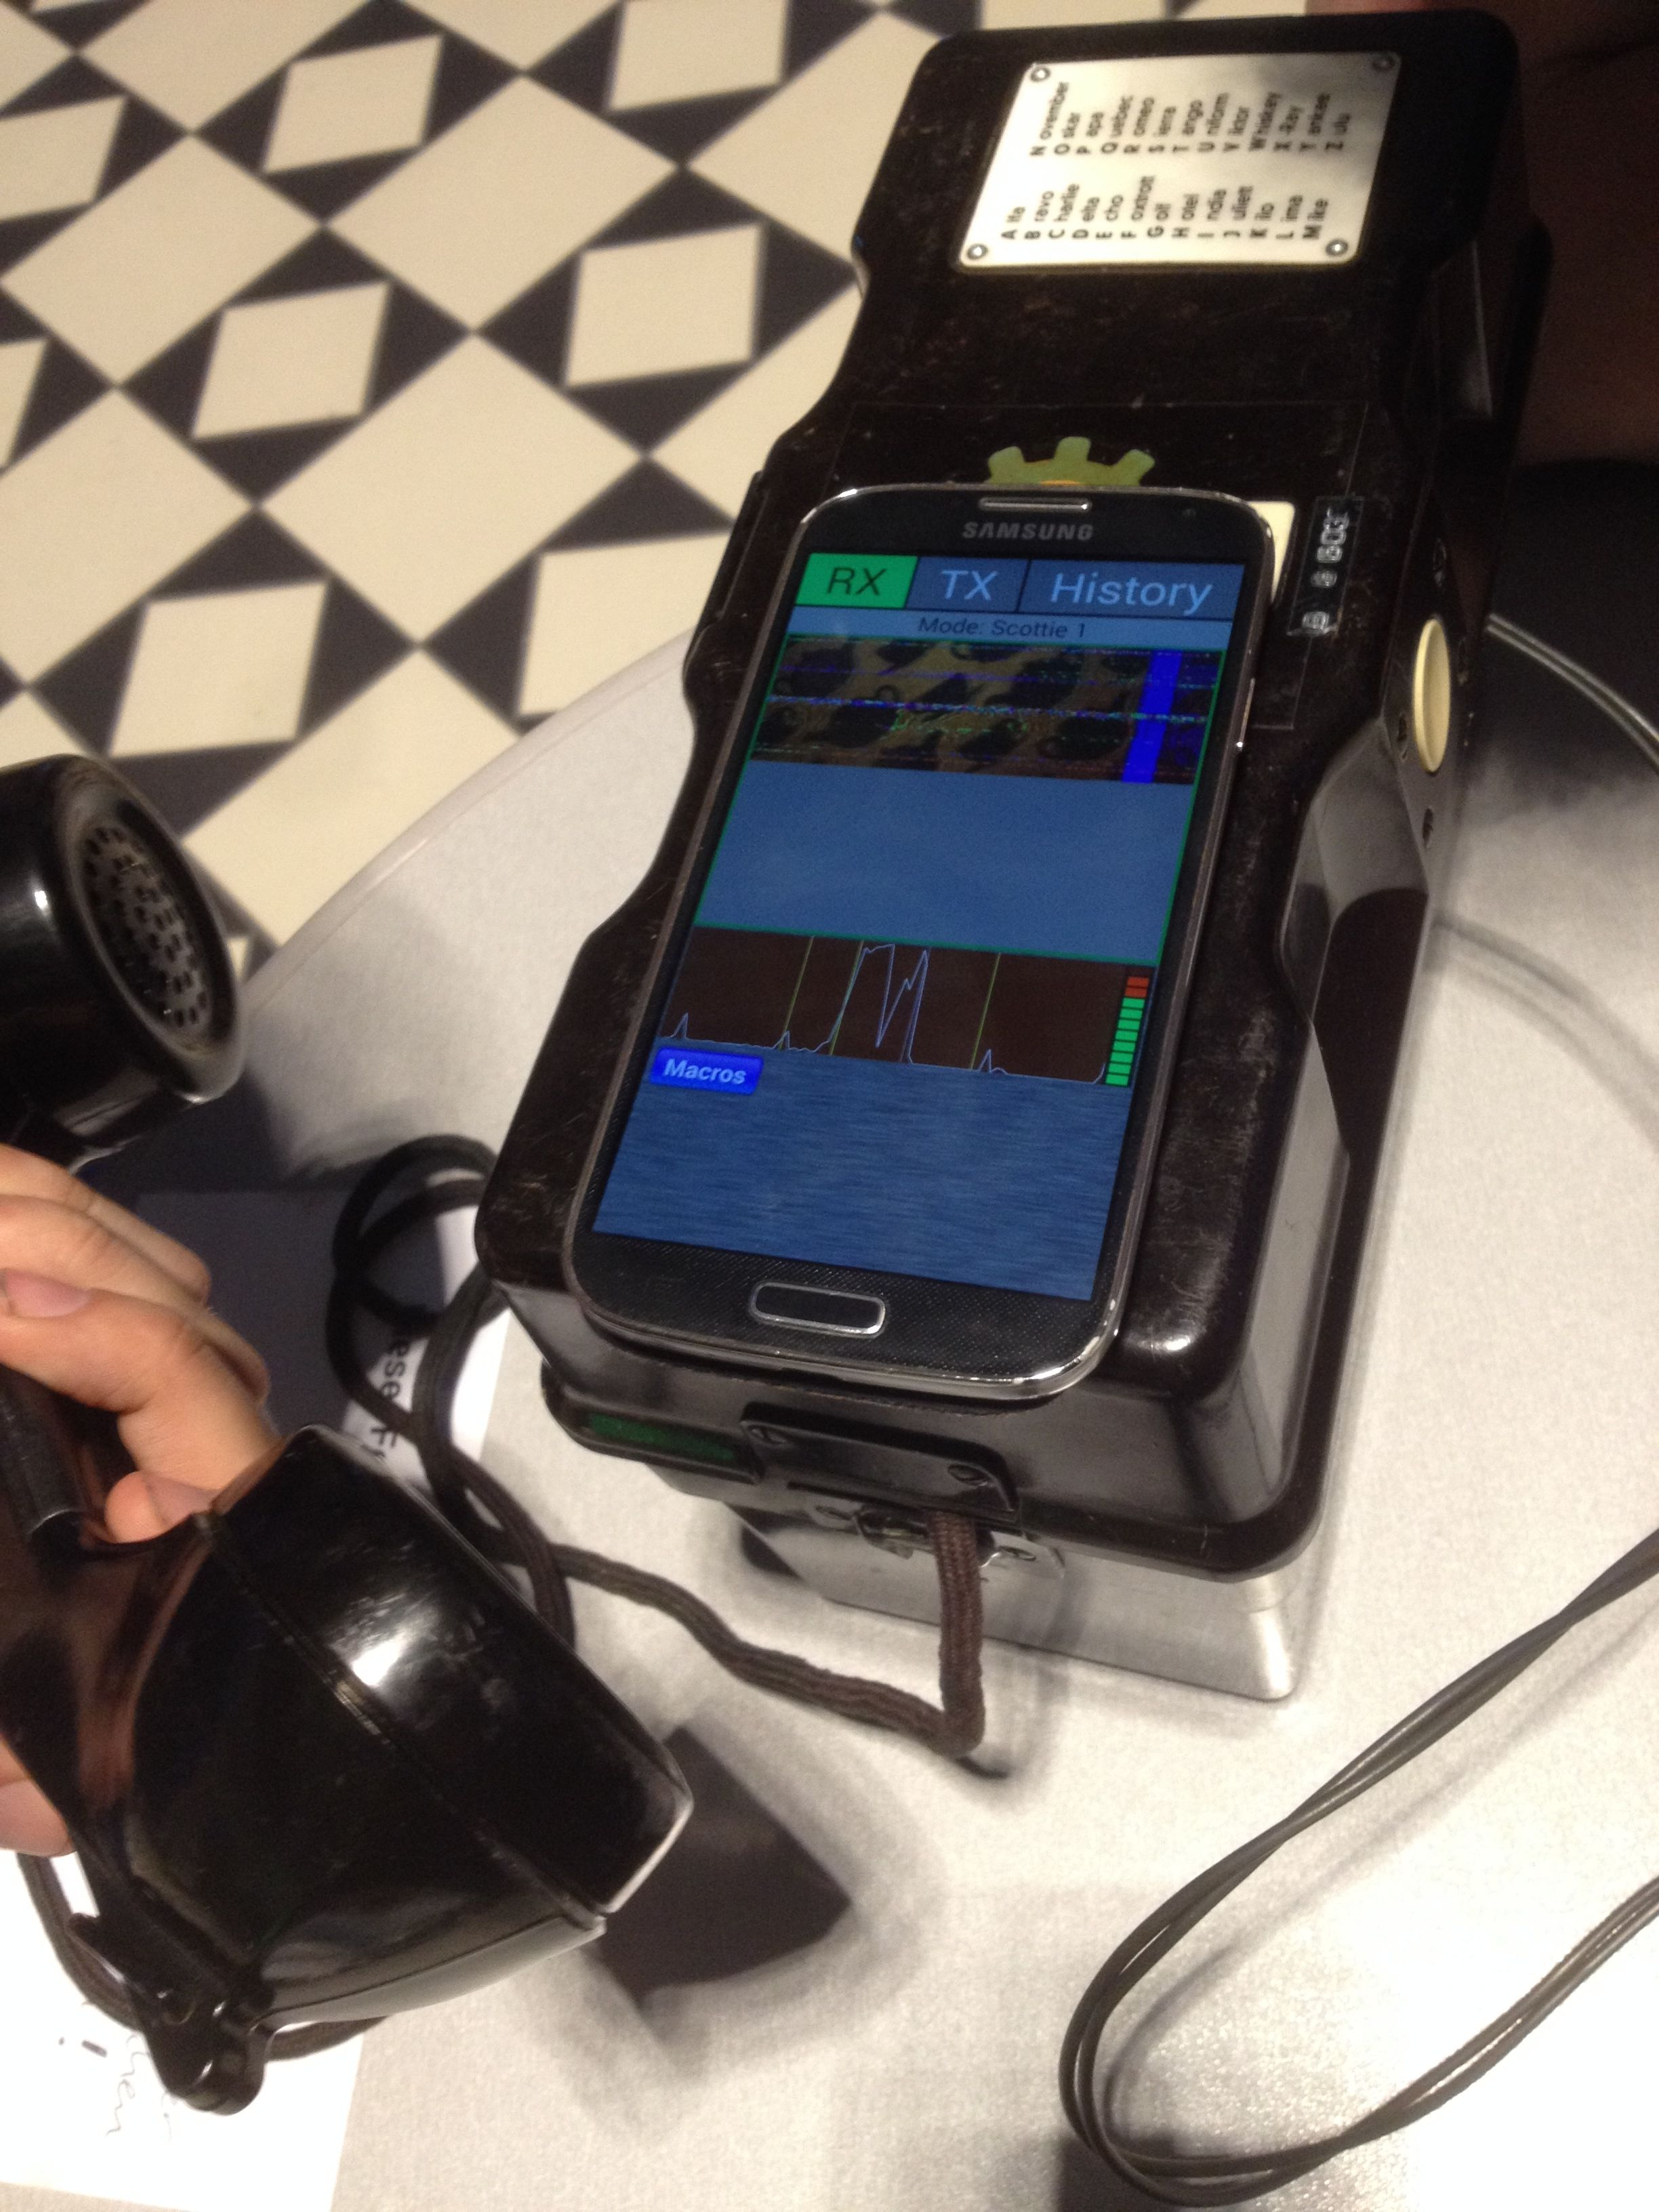
\includegraphics[width=0.5\textwidth,height=.8\textheight,keepaspectratio]{e16/SSTV-over-Ackerschnacker_LNDW2014.jpg}
        \footnote{SSTV über Feldtelefon \emph{Lange Nacht der Wissenschaften} 2014}
    \end{center}

\end{frame}

\begin{frame}
    \frametitle{SSTV / Demo}

    \Large{Ohren gespitzt... es spricht für Sie: \emph{QSSTV}}

\end{frame}

\subsection[ATV]{Amateurfunk-Fernsehen, analog ATV}

\begin{frame}
    \frametitle{ATV}

    Amateurfunk-Fernsehen, analog ATV

    \begin{center}
        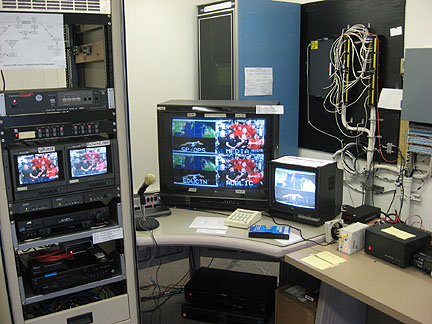
\includegraphics[width=0.6\textwidth,height=.45\textheight,keepaspectratio]{e16/SVECS-atv16.jpg}
        \tiny \hyperlink{refs}{\cite{atv}}
    \end{center}

    \begin{itemize}
        \item technisch wie klassisches analoges Fernsehen
        \item $BW = 6,5 MHz$ -- logischerweise nichts für HF und VHF
        \item auch hier liegt der Fokus inzwischen auf digitaler Übertragung
        \begin{itemize}
            \item Schmalband ATV (\emph{SATV}, $1 MHz$) im Prinzip $\equiv$ \emph{DVB}
        \end{itemize}
    \end{itemize}

\end{frame}

\section{digital}

\subsection[CW]{Morsetelegrafie (CW)}

\begin{frame}
    \frametitle{Morsetelegrafie (CW)}

    \begin{center}
        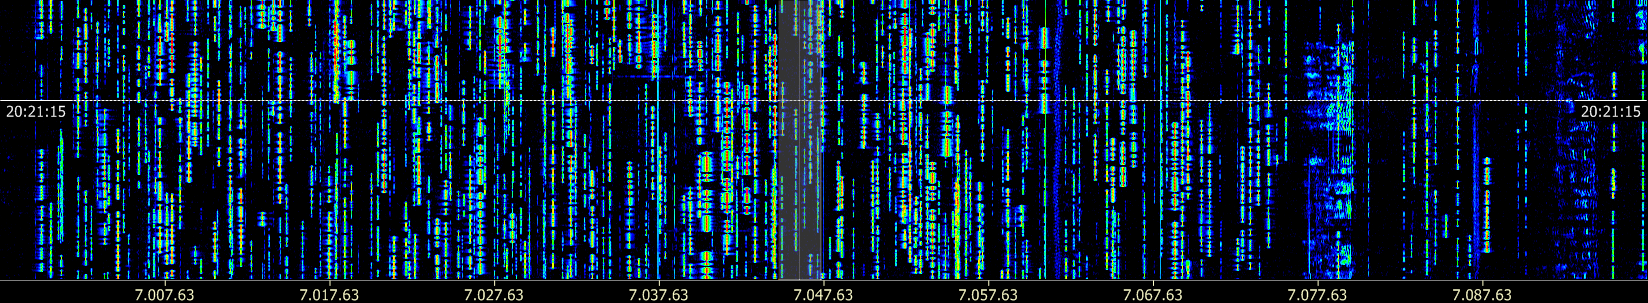
\includegraphics[width=1\textwidth]{e16/CQWW_2013_CW_Waterfall.png}
        \footnote{Wasserfalldiagramm \emph{CQ WW Contest} 2013}
    \end{center}

    \emph{A1A} aka \emph{ASK (amplitude shift keying)} -- die Mutter aller
    Betriebsarten -- ja, digital!

    \begin{itemize}
        \item ``menschenlesbarer'' Digimode mit ausreichend Training
        \item Bandbreite je nach Geschwindigkeit \& Qualität ca. $200-500 Hz$
              \footnote{Interessante Ausführungen zu Bandbreite und SNR von
              DK5KE: \url{http://www.qsl.net/dk5ke/a1a.html}}
              $\rightarrow$ besserer $SNR$ bei gleicher Leistung als z.B. \emph{SSB}
        %\item durch bekannte Abkürzungen einfache QSOs ohne
        %      Fremdsprachenkenntnisse möglich 
    \end{itemize}

\end{frame}

\begin{frame}
    \frametitle{CW / Demo}

    \Large{Ohren gespitzt... es spricht für Sie: \emph{Fldigi}}

\end{frame}

\subsection[RTTY]{Funkfernschreib-Telegrafie (RTTY)}

\begin{frame}
    \frametitle{Funkfernschreib-Telegrafie (RTTY)}

    \textbf{R}adio \textbf{T}ele\textbf{TY}pe

    \begin{center}
        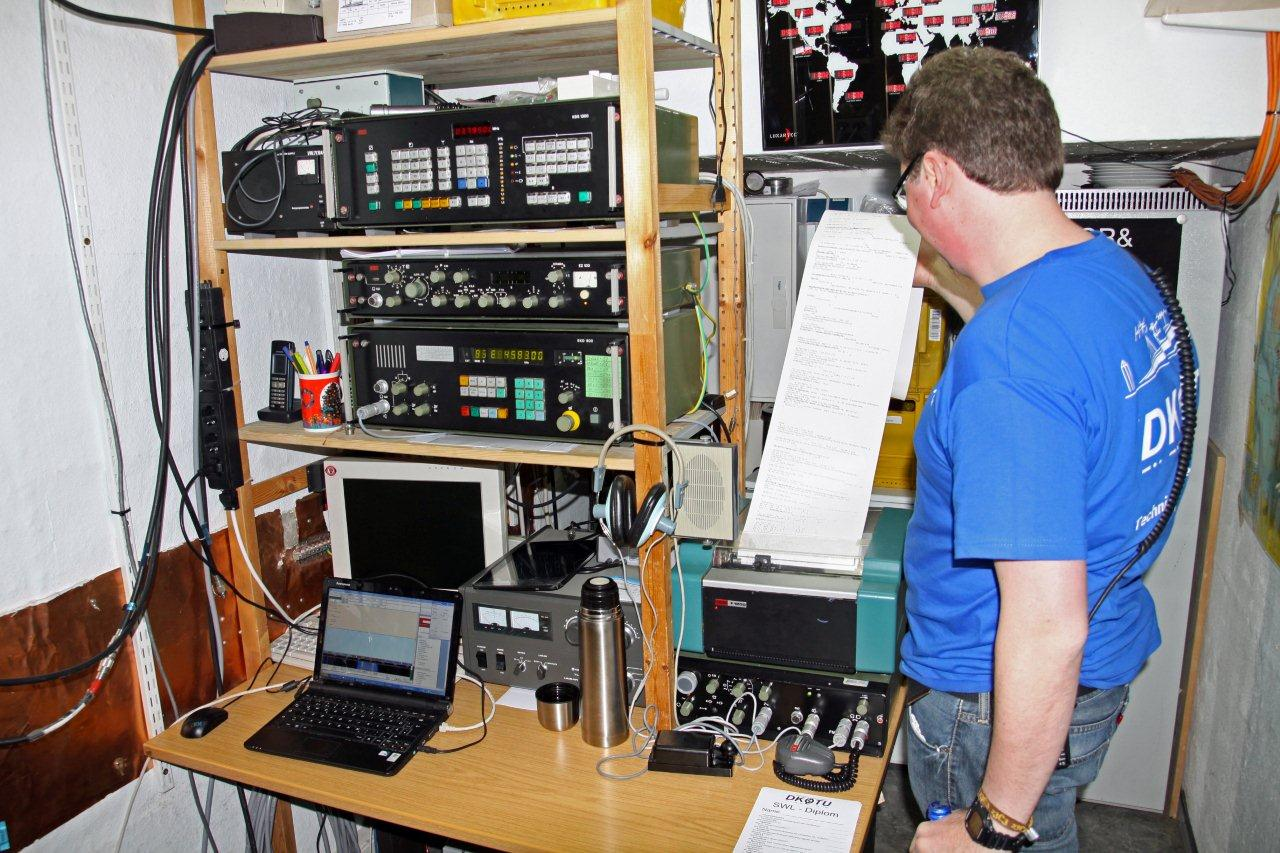
\includegraphics[width=0.5\textwidth,height=.35\textheight,keepaspectratio]{e16/RTTY_LNDW2014.jpg}
        \footnote{RTTY-RX \emph{Lange Nacht der Wissenschaften} 2014}
    \end{center}

    %todo Bild Fernschreiber

    \begin{itemize}
        \item simplex oder semiduplex auf einer Frequenz
        \item früher:
            \begin{itemize}
                \item TX: elektromechanische Fernschreiber mit kontaktierter
                      Schreibmaschinentastatur
                \item RX: Fernschreibdrucker
            \end{itemize}
        \item heute: Software - klar.
    \end{itemize}

\end{frame}

\begin{frame}
    \frametitle{RTTY / Technik}

    \begin{itemize}
        \item fünf Kontakte $\rightarrow$ Baudot 5-Bit-Code, später CCITT-1 bzw. Baudot-Murray-Code CCITT-2
        \item \emph{AFSK}\footnote{Audio Frequency Shift Keying}:
              $2^5 = 32 Bit$ in $0$ und $1$ $\rightarrow$ Mark und Space
        \item Abstand = Shift
        \item Kurzwellenshift 170 Hz, UKW 850 Hz
              % todo Skizze bzw. Screenshot Spektrum
        \item technische Details: Technik Klasse A (A15)
    \end{itemize}

\end{frame}

\begin{frame}
    \frametitle{RTTY / Demo}

    \Large{Ohren gespitzt... es spricht für Sie: \emph{Fldigi}}\\[2em]
    \pause
    Teletype mit Dampf: \url{https://media.ccc.de/v/24c3-2338-en-steam_powered_telegraphy}

\end{frame}

 
\subsection{(B)PSK31}

\begin{frame}
    \frametitle{(B)PSK31}
 
    (\textbf{B}inary) \textbf{P}hase \textbf{S}hift \textbf{K}eying (31)

    \begin{columns}[c]
        \column[c]{8cm}
            \begin{itemize}
                \item BPSK31 eine der Standard-QRP-Betriebsarten
                \begin{itemize}
                    \item zwei Phasenlagen ($0^{\circ}$, $180^{\circ}$)
                    \item Bitrate von $31,25 Bit/s$
                    \item Bandbreite entspricht ca. Bitrate pro Sekunde, $31Hz$
                \end{itemize}
                \item im Vgl. zu CW ca. $\frac{1}{10}$ Bandbreite $\rightarrow$ \\
                      $SNR \approx +10dB$ (Filterung \& selbe Leistung)
                \item Modulation/Demodulation mit Software (Soundcard SDR)
                \item auch QPSK (Quadratur), 8-PSK, ...
            \end{itemize}
        \column{2cm}
        \begin{center}
            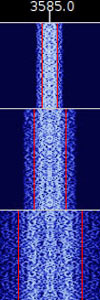
\includegraphics[width=1\textwidth,height=.7\textheight,keepaspectratio]{e16/BPSK_31_63_125.jpg}
            \tiny \hyperlink{refs}{\cite{wc}}
            \scriptsize BPSK31/63/125
        \end{center}
    \end{columns}

\end{frame}

\begin{frame}
    \frametitle{PSK31 / Demo}

    \Large{Ohren gespitzt... es spricht für Sie: \emph{Fldigi}}

\end{frame}

\subsection{Baudrate}

\begin{frame}
    \frametitle{Baudrate}

    Der Vollständigkeit halber: \\[2em]

    \begin{center}
        $1 Bd = 1 \frac{Symbol}{s} = Symboldauer^{-1}$
    \end{center}

    Bei binären Modulationsverfahren entspricht das der Bitrate. Gibt es mehr
    als zwei Symbole ist die Bitrate höher als die Baudrate. Beispiele:

    \begin{itemize}
        \item RTTY: Bitrate = \only<1>?\only<2>1x Baudrate
        \item BPSK31: Bitrate = \only<1>?\only<2>1x Baudrate
        \item BPSK63: Bitrate = \only<1>?\only<2>1x Baudrate
        \item QPSK: Bitrate = \only<1>?\only<2>2x Baudrate
    \end{itemize}

\end{frame}

\subsection{WSJT}

\begin{frame}
    \frametitle{WSJT (FSK441, JT65, JT9)}

    \textbf{W}eak \textbf{S}ignal communication by K1\textbf{JT} \\[2em]

    Gruppe von Übertragungsprotokollen\footnote{Open-Source-Projekt} für
    Soundcard SDR in SSB-Bandbreite, z.B.:
    
    \begin{itemize}
        \item Meteorscatter (schnell): FSK441\footnote{Vierton Frequenzumtastung
              (\emph{FSK}) mit 441 Baud}
        \item EME, Troposcatter (schwache Signale): JT65\footnote{\emph{MFSK
              (Multiple Frequency Shift Keying)} mit 65 Tönen}
        \item Mittel- und Langwelle (schmalbandig): JT9\footnote{ähnlich JT65}
    \end{itemize}

    Mehr dazu unter \url{https://media.ccc.de/v/eh15_-_11_-_de_-_saal_-_201504051730_-_wspr_und_wsjt_-_pylon}

\end{frame}

\begin{frame}
    \frametitle{WSJT / FSK441}

    Beispiel FSK441:

    \begin{itemize}
        \item Zeichen besteht aus nacheinandergesendeten drei von den vier Tönen
        \item Übertragungsgeschwindigkeit 147 Buchstaben/s $\rightarrow$
              \textbf{Meteorscatter}
        \item Ping ca. $\frac{1}{10}s$ (100km über der Erde) $\rightarrow$ 15 Zeichen
        \item 144,370 MHz Anruf-QRG, ab Kontaktaufnahme QSY
        \item Rapporte nach speziellem Kurzzystem
    \end{itemize}

\end{frame}

\subsection{ARQ-Protokolle}

\subsubsection{Verfahren}

\begin{frame}
    \frametitle{ARQ-Protokolle / Verfahren}

    \textbf{A}utomatic \textbf{R}epeat re\textbf{Q}uest

    zuverlässige Datenübertragung durch Sendewiederholungen:

    \begin{itemize}
        \item erfordert ein Verfahren zur Fehlererkennung, z.B. Checksummen
        \item Feedback: \emph{ACK/NAK}-Signale (\emph{Acknowledgement} / {Negative Acknowledgement})
        \item ggf. Wiederholung der Nachricht
    \end{itemize}

    In Kombination mit Kanalcodierung (Hinzufügen von Redundanz, wie z.B.
    \emph{FEC}\footnote{Forward Error Correction}) genauer: Hybride \emph{ARQ-Protokolle}.

\end{frame}

\subsubsection{AMTOR}

\begin{frame}
    \frametitle{AMTOR}

    \textbf{A}mateur \textbf{T}eleprinting \textbf{O}ver \textbf{R}adio

    \begin{itemize}
        \item 1978 veröffentlicht, in der Seefahrt wurden ähnliche Verfahren benutzt
        \item erstes einfaches ARQ-Protokoll nach Schema ``Stop-and-Wait''
        \begin{itemize}
            \item hohe Übertragungssicherheit: in $450ms$-Sendelücke TX von drei
                  Kontrollzeichen ($240ms$) Quittung
            \item ergo: Halbduplexbetrieb auf einer ``Simplex-QRG'' unter
                  Berücksichtigung vom \emph{TX Delay}
        \end{itemize}
        \item Modulation sonst im Prinzip wie RTTY: FSK mit gleichen Tönen und gleicher Shift
        \item allerdings 7-Bit-Code und Geschwindigkeit 100 Baud
        \item implementiert auch bereits eine \emph{FEC}
    \end{itemize}

\end{frame}

\subsubsection{AX.25}

\begin{frame}
    \frametitle{AX.25}

    8-Bit-Standard\footnote{1984 v2.0 standardisiert} für Pakete (Frames) mit Adressierung und Prüfsumme:

    \begin{center}
        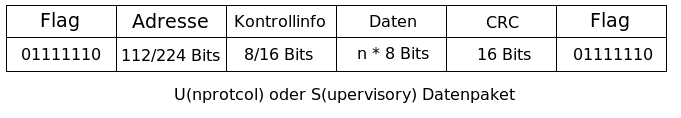
\includegraphics[width=1\textwidth]{e16/Ax25-US-Paket.png}
        \tiny \hyperlink{refs}{\cite{wc}}
    \end{center}

    \begin{itemize}
        \item Sicherungsschicht (Data Link Layer)
              \footnote{\emph{OSI (Open Systems Interconnection Model)}-Layer 2}
        \item Anpassung des  \emph{ITU-T X.25}-Standards (Layer
              1-3)\footnote{Bitübertragungsschicht, Sicherungsschicht,
              Vermittlungsschicht} aus den 1970ern
        \item verbindungsorientiert, aber Übertragung von verbindungslosen Daten zulässig
    \end{itemize}

\end{frame}

\subsubsection {Packet Radio (PR)}

\begin{frame}
    \frametitle{Packet Radio (PR)}

    Paketbasiertes ``Radio'' - Grundlage: \emph{AX.25}
        
    \begin{itemize}
        \item Kennt einer (noch) \emph{GPRS}?
    \end{itemize}
   
\end{frame}

\begin{frame}
    \frametitle{Packet Radio / Technische Grundlagen (Duplex)}

    Duplex (Zeit- und ggf. Frequenzduplex), mit Fehlerkorrektur
    %todo http://de.wikipedia.org/wiki/Duplex_%28Nachrichtentechnik%29
    %todo Wiederholung Kapitel BV11: Simplex, HD, Duplex mit Skizze

    \begin{itemize}
        \item mehrere Stationen auf einer \emph{QRG} (Timeslots)
        \item verschiedene Hin- und Rückfrequenzen möglich \\ $\rightarrow$
              Unterscheidung:
        \begin{itemize}
            \item Simplex\footnote{Afu-Simplex ``Senden bzw. Empfangen auf
                  der gleichen Frequenz''!}-Digipeater (Halbduplex, selbe QRG)
            \item Duplex-Digipeater (2 QRGs\footnote{70-cm: Ablage $7,6 MHz$
                  oder $9,4 MHz$ höher})
        \end{itemize}
        \item Digipeater-``User'' im Halbduplex:
        \begin{itemize}
            \item RX (Ausgabefrq.)
            \item TX (Eingabefrq.)
        \end{itemize}
    \end{itemize}

\end{frame}

\begin{frame}
    \frametitle{Packet Radio / Technische Grundlagen (Baudraten)}

    Viel höhere Datenraten als RTTY:

    \begin{itemize}
        \item \textbf{1k2 Bd}: AFSK\footnote{$1200$ \& $2200 Hz$}-Subträger \\
              (Bandbreite 1x $12,5kHz$-Kanal, NF-BW $3000 Hz$)
        \item \textbf{9k6 Bd}: FSK direkt aufmoduliert
              \footnote{Leitungscodierung ist auch anders (Manchester-Code?)} \\
              (Bandbreite 20kHz $\rightarrow$ 1x $25kHz$-Kanal)
              %todo Skizzen der Bandbreiten von DJ4UF?
              %     http://www.darc.de/referate/ajw/ausbildung/darc-online-lehrgang/technik-klasse-e/technik-e16/#Packet-Radio
    \end{itemize}

    $\rightarrow$ VHF/UHF (eher unüblich: HF $300 Bd$)

\end{frame}

\begin{frame}
    \frametitle{Packet Radio / Packaging}

    Zusammensetzen der Pakete am Ziel zur Nachricht \\[1em]

    \begin{itemize}
        \item Leerzeiten ohne Aussendung, kann von anderen Stationen genutzt werden
        \begin{itemize}      
            \item eine Übertragungsstrecke für viele gleichzeitige Verbindungen
        \end{itemize}
        \item Problem: Kollisionen verschiedener Pakete trotz
              ``sensing''\footnote{wenn QRG frei: TX}
        \item Lösungen:
        \begin{itemize}
            \item zufällige Wartezeit beider TX
            \item DAMA\footnote{Demand Assigned Multiple Access}: Digipeater fragt Stationen ab
            \begin{itemize}
                \item Overhead, aber Kollisionen werden vollständig vermieden
            \end{itemize}
        \end{itemize}
    \end{itemize}

\end{frame}

\begin{frame}
    \frametitle{Packet Radio / Vernetzung \& Routing}

    Netzstruktur durch Digipeater\footnote{``unbesetzte, fernbediente feste
    Amateurfunkstellen für Packet Radio''} (Digital Repeater), digitale
    Zwischenstationen/Relais

    \begin{itemize}
        \item teilweise mit ``Linkstrecken''\footnote{Prüfungsfrage:
              ``Linkstrecken sind fest eingerichtete Funkverbindungen zur
              Vernetzung von Relaisfunkstellen oder Digipeatern.''} oder
              weltweit (Internet \& Co) untereinander vernetzt
        \item Datenpakete von Sender zu Empfänger und ggf weiter im Verbindungsnetz
        \item es gibt z.B.
        \begin{itemize}
            \item Speicher für Nachrichten (Mailboxen)
            \item DX-Cluster via \texttt{telnet}
            \item IRC Channel
        \end{itemize}
    \end{itemize}

\end{frame}

\begin{frame}
    \frametitle{Packet Radio / Vernetzung \& Routing}

    Fragen an unsere ``Digital Natives'': \\[2em]

    \begin{exampleblock}{Wozu dient ein ``Auto-Router'' im Packet-Radio-Betrieb?}
      \only<1>{\vspace{1em}}
      \only<2>{Eine Einrichtung, die es ermöglicht automatisch ein Zielrufzeichen zu erreichen.}
    \end{exampleblock}
    \begin{exampleblock}{Was versteht man unter ``Forwarding'' im
      Packet-Radio-Betrieb?}
      \only<1>{\vspace{1em}}
      \only<2>{Automatisches Weiterleiten von Nachrichten an andere Mailboxen}
    \end{exampleblock}

\end{frame}

\begin{frame}
    \frametitle{Packet Radio / Begriffe}

    \begin{block}{Zum Merken: Begriffe im Amateurfunk-Sprachgebrauch}
        \begin{description}
            \item[Repeater] \only<2>{unbesetzte, fernbediente feste
                                     Amateurfunkstellen für Telefoniebetrieb}
            \item[Digipeater] \only<2>{unbesetzte, fernbediente feste
                                       Amateurfunkstellen für Packet Radio}
            \item[Mailbox] \only<2>{Datenbank mit allgemeinen Zugriff zum
                                    Abspeichern und Auslesen von Informationen}
            \item[Relais] \only<2>{Funkstelle zur Umsetzung von Funksignalen}
        \end{description}
    \end{block}

\end{frame}

\begin{frame}
    \frametitle{Packet Radio / Praxis}

    Man braucht: PTT, TX, RX -- Hardware-MODEM und Controller, ein \emph{TNC
    (Terminal Node Controller)} oder Software-\emph{TNC} \\[2em]

    %todo Bild TNC bzw. Blockschaltbild Setup - interaktiv an Tafel ging aber bisher

    \begin{block}{TX-Delay des PTT $50$ bis $250ms$ - Wozu?}
      \only<1>{\vspace{3em}}
        \only<2>{
        \begin{itemize}
            \item so kurz wie möglich, sonst wird Übertragungszeit verschwendet --
                  ökonomische Nutzung der Kanalkapazität auf der Frequenz
            \item so lang wie nötig, da sonst Daten bei der Umschaltung ``verschluckt''
                  werden
        \end{itemize}
        }
    \end{block}

\end{frame}

\subsubsection{APRS}

\begin{frame}
    \frametitle{APRS}

    \textbf{A}utomatic \textbf{P}acket \textbf{R}eporting \textbf{S}ystem

    \begin{center}
        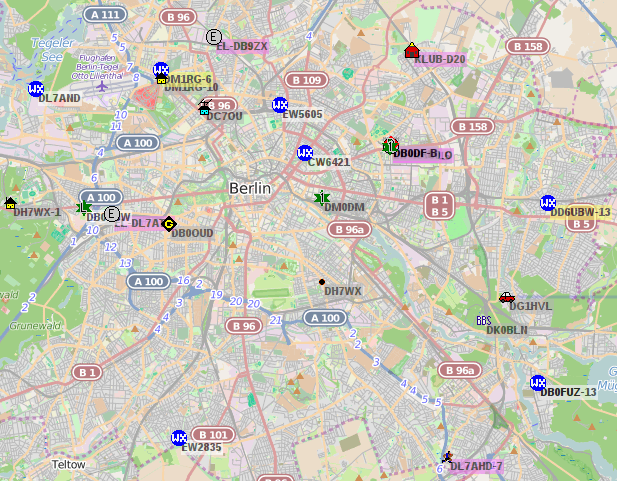
\includegraphics[width=0.5\textwidth,height=.4\textheight,keepaspectratio]{e16/APRS.png}
        \footnote{\url{http://aprs.fi} Screenshot vom 22.01.2015}
    \end{center}

    \begin{itemize}
        \item Positionsmeldungen, Wetterdaten, Messwerte, ...
        \item Modulation Packet Radio, in ``echtes Simplex''
        \item Backbone: Packet Radio Digipeater-Netzwerk bis zum erreichen eines
              APRS-Digipeaters
    \end{itemize}

\end{frame}

\begin{frame}
    \frametitle{APRS}

    \begin{center}
        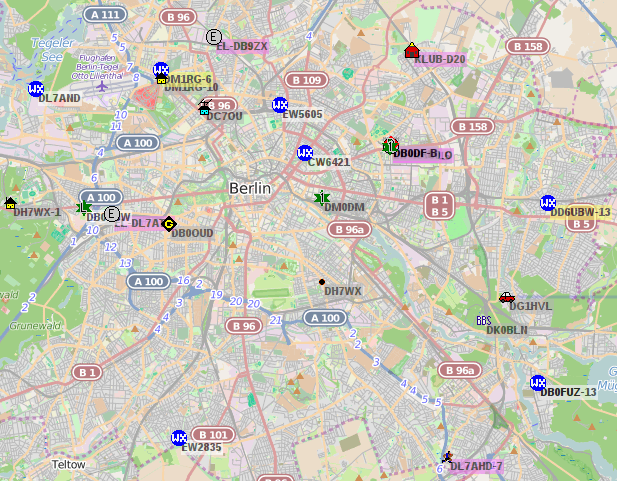
\includegraphics[width=0.8\textwidth,height=.8\textheight,keepaspectratio]{e16/APRS.png} \\
        \Large Demo!
    \end{center}

\end{frame}

\subsubsection{ARQ Heute}

\begin{frame}
    \frametitle{ARQ Heute}

    Hervorgegangen aus \emph{AMTOR} und \emph{Packet Radio}, auf Kurzwelle z.B.
    \emph{PACTOR}\footnote{\textbf{PAC}ket \textbf{T}eleprinting \textbf{O}ver
    \textbf{R}adio} und \emph{WINMOR}\footnote{\textbf{Win}Link \textbf{M}ail
    \textbf{O}ver \textbf{R}adio}

    \begin{itemize}
        \item 8 Bit als Basis für alle Betriebsarten
        \item + verschiedene Fehlerkorrekturverfahren
        \item + verschiedene Modulationsarten je nach Kanaleigenschaften
        \item auch bei sehr schwachen Signalen im Rauschen noch nutzbar
    \end{itemize}

    \vspace{0.5cm}

    \emph{PACTOR} Rant: Man braucht einen teuren TNC, der
    gebrauchsmustergeschützt ist -- Selbstbau nicht (mehr) möglich.

\end{frame}

\begin{frame}
    \frametitle{ARQ Heute / Netzwerke}

    \begin{itemize}
        \item globales HF-Mailboxsysteme mit der Möglichkeit Forwarding per
              Internet-E-Mail, z.B. \emph{WinLink2000}
        \item \emph{HAMNET (Highspeed Amateurradio Multimedia NETwork)} benutzt
              \emph{IEEE 802.11}-Technologie im $GHz$-Bereich
    \end{itemize}

    \begin{center}
        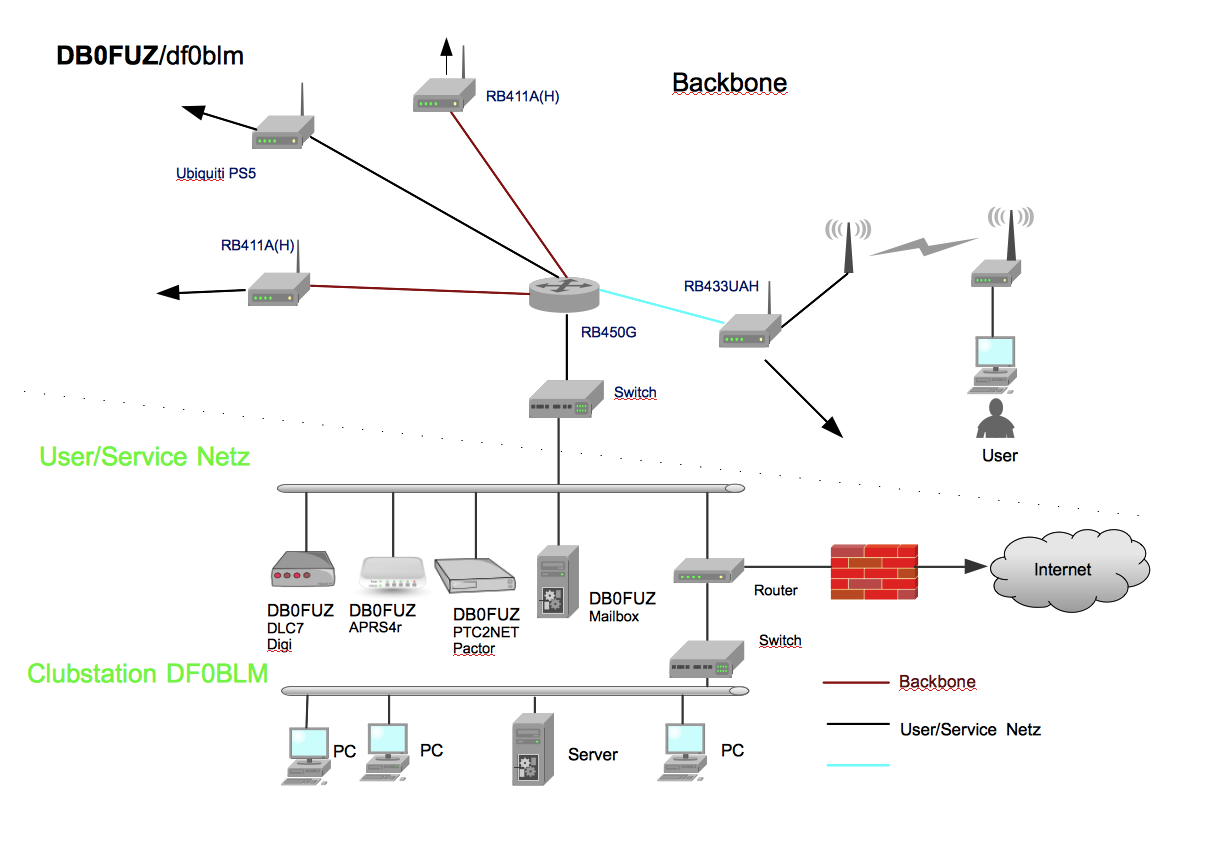
\includegraphics[width=0.6\textwidth,height=.55\textheight,keepaspectratio]{e16/db0fuz.png}
        \tiny \hyperlink{refs}{\cite{db0fuz}}
    \end{center}

\end{frame}

\begin{frame}
    \frametitle{ARQ Heute / WinLink2000}

    \begin{center}
        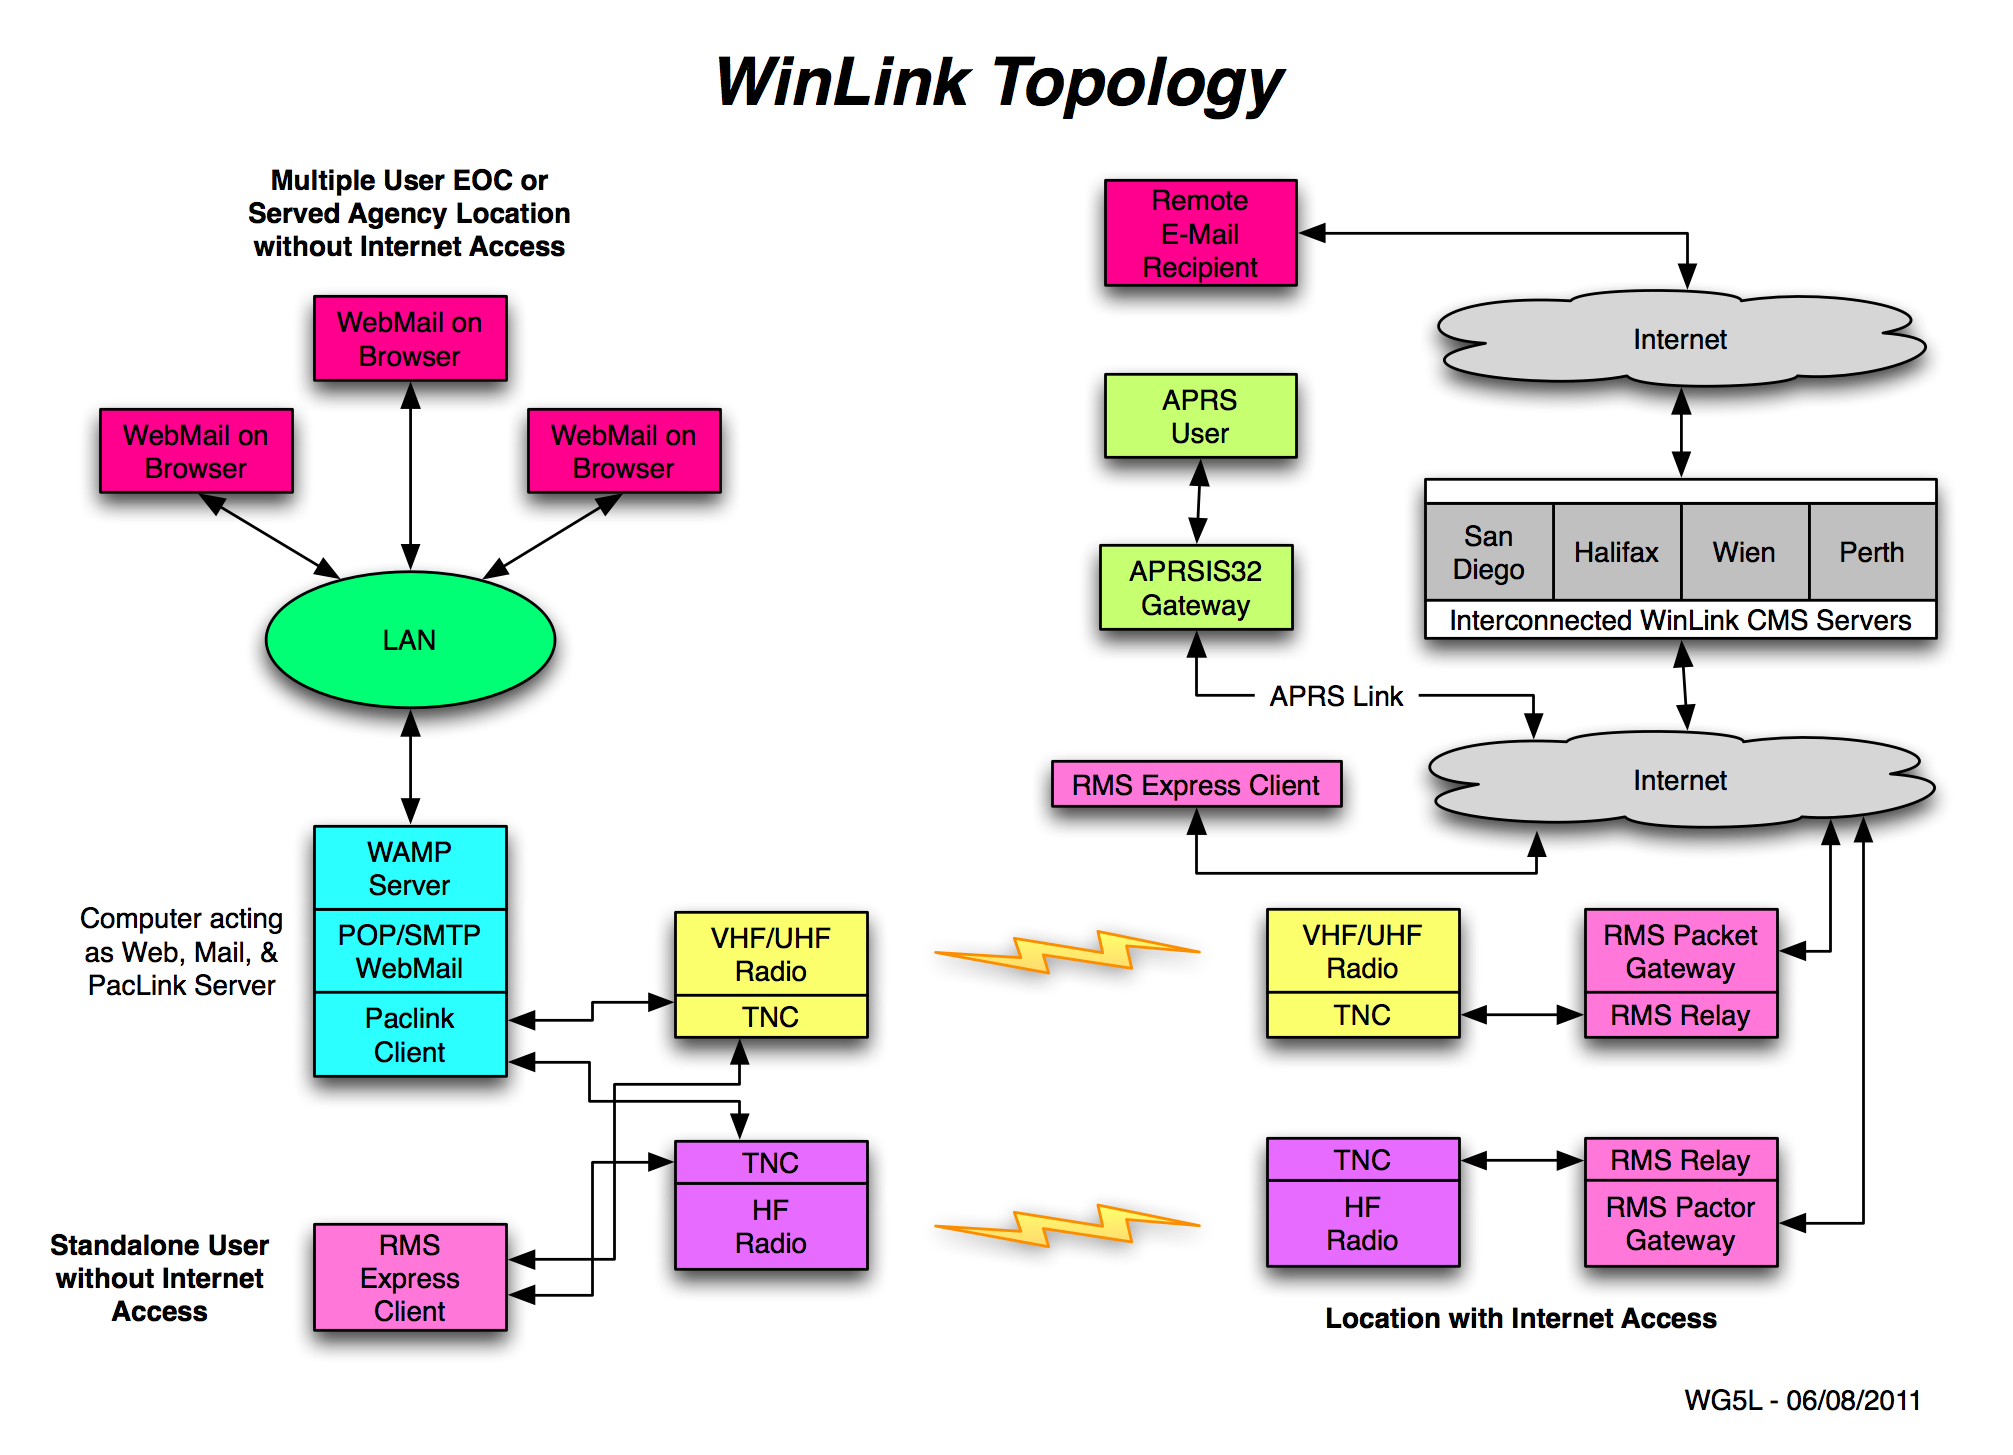
\includegraphics[width=.8\textwidth,height=.85\textheight,keepaspectratio]{e16/WinLink_Topology.jpg}
        \tiny \hyperlink{refs}{\cite{wl2k}}
    \end{center}

\end{frame}

\begin{frame}
    \frametitle{ARQ Heute / HAMNET}

    \begin{center}
        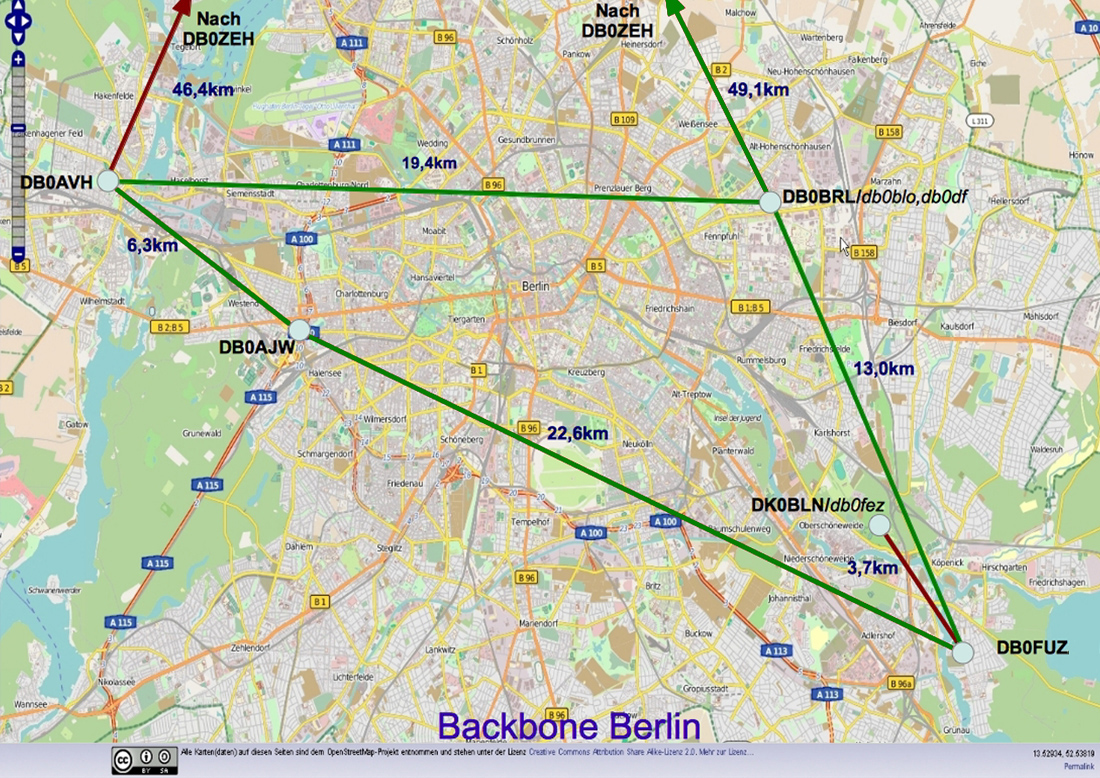
\includegraphics[width=.8\textwidth,height=.75\textheight,keepaspectratio]{e16/backbone_berlin1201.jpg}
        \footnote{\url{http://hamnet.funkzentrum.de} (Stand 24.03.2012)}
    \end{center}

\end{frame}

\subsection{Sprechfunk}

\begin{frame}
    \frametitle{Sprechfunk (digital)}

    %todo ausbauen

    Der Vollständigkeit halber: Digitale Betriebsarten für den Sprechfunk gibt
    es zunehmend, z.B. \emph{FreeDV}\footnote{Free Digital Voice} für Kurzwelle oder \emph{DMR}\footnote{Digital Mobile Radio} für UHF/VHF.

\end{frame}

\subsection{Zusammenfassung}

\begin{frame}
    \frametitle{Zusammenfassung}

    \begin{center}
        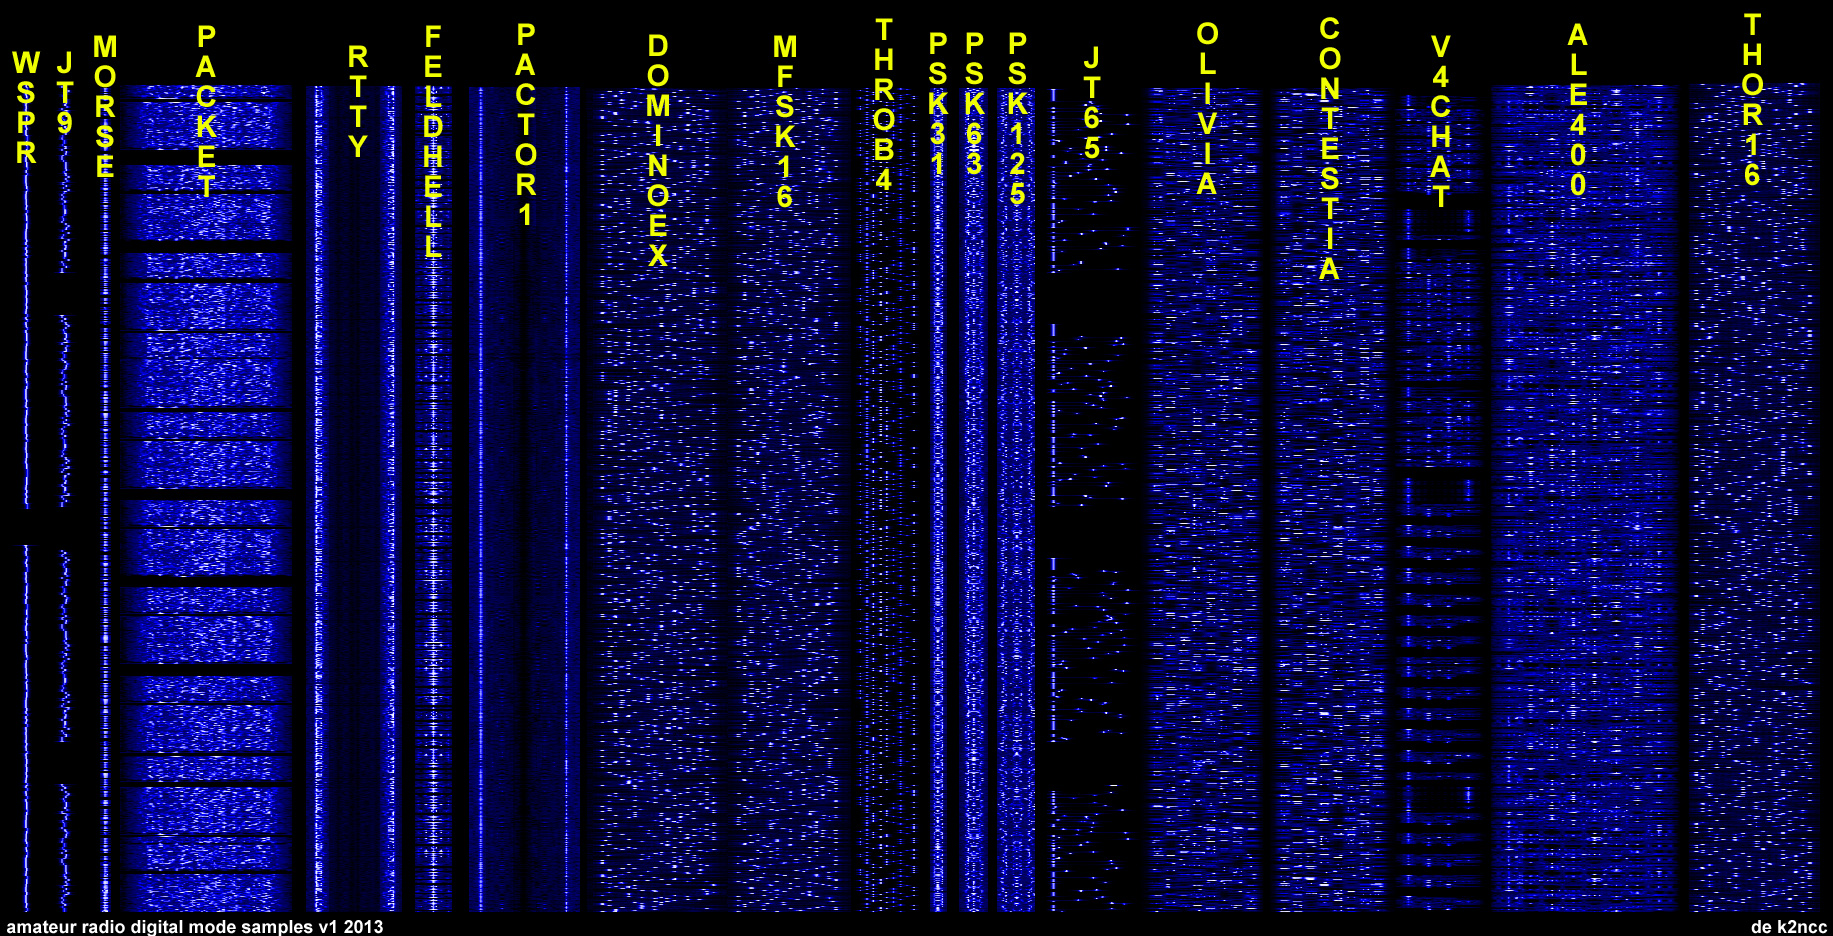
\includegraphics[width=.85\textwidth,height=.85\textheight,keepaspectratio]{e16/Digital_Rosetta_Stone.jpg}
        \footnote{``Digital Rosetta Stone'' by K2NCC}
    \end{center}

\end{frame}

\section{Quiz}

\begin{frame}
    \frametitle{Quiz}

    \begin{exampleblock}{Welche Betriebsarten sind für QRP-DX-Betrieb auf Kurzwelle am
    besten geeignet?}
    \only<1>{\vspace{3em}}
        \only<2>{In den Prüfungsantworten: CW, Pactor, PSK31
        \begin{itemize}
            \item Bandbreiten?
            \item Wie viele habt ihr herausgefunden?
        \end{itemize}
        }
    \end{exampleblock}

% todo Aufgabe Nach Bandbreite sortieren?
%     * Telegrafie benötigt u.U. weniger als 200 Hz Bandbreite
%     * PSK31, MSK63, JT65                                    
%     *alle die vorher dran waren

% todo Jeopardy Sektion zu Betriebsarten (Spektrum und Bandbreiten) machen

\end{frame}

\section{NF-QSOs}

\begin{frame}
    \frametitle{NF-QSOs: Fldigi, QSSTV, ...}

    \Large \textbf{Pause.}
    \normalsize Anschließend Erklärung der Bedienung. \\[2em]

    %todo Screenshots der Programme

    Wer die Tools nicht installiert hat, nutzt die Zeit. ;-)

    %todo WSJT, ARQ-Protokolle und FreeDV via NF testen?
    %     ... Vielleicht bei Klasse A dann.

\end{frame}

\renewcommand{\refname}{Referenzen}

\hypertarget{refs}{}
\textcolor{white}{} \\ %\vspace{} geht nicht
\Large Referenzen/Links
\footnotesize

\begin{thebibliography}{}
    \setbeamertemplate{bibliography item}[online]
    \bibitem{bv12}  Moltrecht B/V 12: \\
                    \url{http://www.amateurfunkpruefung.de/lehrg/bv12/bv12.html}
    \bibitem{e16}   Moltrecht E 16: \\
                    \url{http://www.darc.de/referate/ajw/ausbildung/darc-online-lehrgang/technik-klasse-e/technik-e16/}
    \bibitem{wp}    Wikipedia DE: \\
                    \url{https://de.wikipedia.org/wiki/Einseitenbandmodulation}\\
                    \url{http://de.wikipedia.org/wiki/Slow_Scan_Television}\\
                    \url{http://de.wikipedia.org/wiki/MT63}\\
                    \url{http://de.wikipedia.org/wiki/Amateurfunk-Fernsehen}\\
                    \url{http://de.wikipedia.org/wiki/PSK31}\\
                    \url{https://de.wikipedia.org/wiki/Baud}\\
                    \url{https://de.wikipedia.org/wiki/WSJT}\\
                    \url{http://de.wikipedia.org/wiki/ARQ-Protokoll}\\
                    \url{http://de.wikipedia.org/wiki/AMTOR}\\
                    \url{http://de.wikipedia.org/wiki/AX.25}
    \bibitem{we}    Wikipedia EN: \\
                    \url{https://en.wikipedia.org/wiki/Terminal_node_controller}
    \bibitem{wc}    Wikimedia Commons \\
                    \url{http://commons.wikimedia.org/wiki/File:Ssb-de.png}\\
                    \url{http://commons.wikimedia.org/wiki/File:Dpx-fm-radio.png}\\
                    \url{http://commons.wikimedia.org/wiki/File:Mechanical_glow_drum_slow_scan_television_monitor.gif}\\
                    \url{http://commons.wikimedia.org/wiki/File:Sstv_frequences.svg}\\
                    \url{http://commons.wikimedia.org/wiki/File:SSTV_signal.jpg}\\
                    \url{http://commons.wikimedia.org/wiki/File:BPSK_31_63_125.jpg}\\
                    \url{http://commons.wikimedia.org/wiki/File:Ax25-US-Paket.png}
    \bibitem{atv}   \url{http://www.svecs.net/SVECS-atv16.JPG}
    \bibitem{wl2k}  \url{http://letarc.org/main/2011/06/08/packet-modes-and-winlink-2000/}
    \bibitem{db0fuz}\url{http://hamnet.funkzentrum.de/berliner-hamnet/backbone/hamnet-knoten.html}
    \bibitem{snd}   \url{http://www.nonstopsystems.com/radio/radio-sounds.html}

\end{thebibliography} 

% Hier könnte noch eine Kontaktfolie stehen

\end{document}

